\documentclass[11pt]{article}

\usepackage[margin=1in]{geometry}                                              
\usepackage{amsmath,amsthm,amssymb}  
                                          
\usepackage{graphicx}                                      
\graphicspath{{../figures/}, {../figures/growthrates/}, {../figures/correlations/}}  
\usepackage{titlesec}                                                          
\usepackage{savetrees}                                                         
\usepackage{bm}

\titleformat{\subsection}[runin]
{\normalfont\large\bfseries}{\thesubsection}{1em}{}

\renewcommand{\bf}{\mathbf}
\renewcommand{\cal}{\mathcal}
\newcommand{\pd}[2]{\frac{\partial #1}{\partial #2}}
\newcommand{\pdn}[3]{\frac{\partial^{#3} #1}{\partial #2^{#3}}}
\newcommand{\pdop}[1]{\frac{\partial}{\partial #1}}
\newcommand{\nd}[2]{\frac{d #1}{d #2}}
\newcommand{\ndn}[3]{\frac{d^{#3} #1}{d #2^{#3}}}
\newcommand{\ndop}[1]{\frac{d}{d #1}}
\newcommand{\dt}{\frac{d}{dt}}
\newcommand{\grad}{\bm\nabla}
\newcommand{\cross}{\times}
\newcommand{\curl}{\grad\cross}
\newcommand{\imp}{\Longrightarrow\quad}
\newcommand{\abs}[1]{\left|#1\right|}
\newcommand{\half}{\frac{1}{2}}
\newcommand{\third}{\frac{1}{3}}
\renewcommand{\th}[1]{\frac{1}{#1}}
\renewcommand{\k}{4\pi\epsilon_0}
\newcommand{\eps}{\epsilon_0}
\newcommand{\intt}{\int_{t_1}^{t_2}}
\newcommand{\inti}{\int_{-\infty}^{+\infty}}
\newcommand{\ex}[1]{\left\langle #1 \right\rangle}
\newcommand{\oom}[1]{\times 10^{#1}}
\renewcommand{\d}{\delta}
\renewcommand{\t}{\tau}
\newcommand{\e}{\text{e}}
\renewcommand{\l}{\ell}
\newcommand{\om}{\omega}
\newcommand{\h}{\hbar}
\newcommand{\ket}[1]{\left|#1\right\rangle}
\newcommand{\bra}[1]{\left\langle#1\right|}
\newcommand{\braket}[2]{\left\langle#1\middle|#2\right\rangle}
\newcommand{\brakett}[3]{\left\langle#1\middle|#2\middle|#3\right\rangle}
\newcommand{\nn}{\nonumber\\}

\begin{document}

\title{Intersession Updates}
\author{Charles Stahl}

\maketitle

\section{3-Site Hamiltonian} \emph{}

We want a three-state Hamltonian that will transport individual states around after a discrete time, such that $\ket{s_2(\t)} = \ket{s_1(0)},\,\ket{s_3(\t)} = \ket{s_2(0)}$, etc, where $\ket{s_a(t)}$ is the state of spin $a$ at time $t$. We can rescale time (equivalently energy) so that a system that starts in state $\ket{\psi_1(0)\psi_2(0)\psi_3(0)}$ becomes
\begin{align}
\ket{s_1(1)s_2(1)s_3(1)} = U(1)\ket{s_1(0)s_2(0)s_3(0)} 
	= \ket{s_3(0)s_1(0)s_2(0)},\label{eqn:condition}
\end{align}
with $U(t)$ being the time evolution operator for time $t$.

There are four states that should not change in time and therefore have 0 energy. Before normalization these are
\begin{align}
\ket{000},\quad \ket{100}+\ket{010}+\ket{001},\nn
\ket{111},\quad \ket{011}+\ket{101}+\ket{110}.\label{eqn:zero}
\end{align}
Of the four other states, two should have positive energy and two should have negative energy. Since $U(3)=1$, their energies should be $E_\pm = \pm\frac{2\pi}{3}$ so they pick up a phase $\phi_\pm =\e^{-iE_\pm} = \e^{\mp i\frac{2\pi}{3}}$. Using condition~\ref{eqn:condition}, we can show that the positive energy states are
\begin{align}
&\ket{100} + \phi_-\ket{010} + \phi_+\ket{001},\nn
&\ket{011} + \phi_-\ket{101} + \phi_+\ket{110},\label{eqn:plus}
\end{align}
while the negative energy states are 
\begin{align}
&\ket{100} + \phi_+\ket{010} + \phi_-\ket{001},\nn
&\ket{011} + \phi_+\ket{101} + \phi_-\ket{110}.\label{eqn:minus}
\end{align}

In matrix notation, with basis states $\ket{000},\,\ket{001},\,\ket{010},$ etc, the hamiltonian is 
\begin{align}
H = T\; \text{diag}(0,0,0,0,E_+,E_+,E_-,E_-)\; T^\dag,
\end{align}
where $T$ is the transformation matrix suggested by~\ref{eqn:zero}, \ref{eqn:plus}, and~\ref{eqn:minus},
\begin{align}
T = \th{\sqrt{3}}\begin{bmatrix}
	\sqrt{3} & 0 & 0 & 0        & 0      & 0      & 0      & 0      \\
	0        & 1 & 0 & 0        & \phi_+ & 0      & \phi_- & 0      \\
	0        & 1 & 0 & 0        & \phi_- & 0      & \phi_+ & 0      \\
	0        & 0 & 1 & 0        & 0      & 1      & 0      & 1      \\
	0        & 1 & 0 & 0        & 1      & 0      & 1      & 0      \\
	0        & 0 & 1 & 0        & 0      & \phi_- & 0      & \phi_+ \\
	0        & 0 & 1 & 0        & 0      & \phi_+ & 0      & \phi_- \\
	0        & 0 & 0 & \sqrt{3} & 0      & 0      & 0      & 0
	\end{bmatrix}
\end{align}
Altogether
\begin{align}
H = \frac{2\pi i}{\sqrt{3}}\begin{bmatrix}
	0 & 0  & 0  & 0  & 0  & 0  & 0  & 0 \\
	0 & 0  & 1  & 0  & -1 & 0  & 0  & 0 \\
	0 & -1 & 0  & 0  & 1  & 0  & 0  & 0 \\
	0 & 0  & 0  & 0  & 0  & -1 & 1  & 0 \\
	0 & 1  & -1 & 0  & 0  & 0  & 0  & 0 \\
	0 & 0  & 0  & 1  & 0  & 0  & -1 & 0 \\
	0 & 0  & 0  & -1 & 0  & 1  & 0  & 0 \\
	0 & 0  & 0  & 0  & 0  & 0  & 0  & 0 \\
	\end{bmatrix}
\end{align}

This hamiltonian should be symmetric under a simultaneous rotation of all three spins, so that it can be written as $H(\bm{\sigma}_1,\,\bm{\sigma}_2 ,\,\bm{\sigma}_3)$. It should be antisymmetric under the interchange of any two spins (equivalent to reversing the direction of propagation). The only function of three vectors that has this property is the triple product $H = \bm{\sigma}_1\cdot\left(\bm{\sigma}_2 \times\bm{\sigma}_3\right)$.

%Note that this is equivalent to
%\begin{align}
%H &= \bm{\sigma}_1\cdot\left(\bm{\sigma}_2 \times\bm{\sigma}_3\right) \nn
%&= \sigma_{1,1}\otimes\sigma_{2,2}\otimes{\sigma}_{3,3} - {\sigma}_{1,1}
%	\otimes\sigma_{2,3}\otimes\sigma_{3,2} + \sigma_{1,2}\otimes{\sigma}_{2,3} \otimes {\sigma}_{3,1}-\cdots
%\end{align}

Exponentiating the hamiltonian gives the time evolution operator for one time step
\begin{align}
U(1) = \e^{-iH} = \begin{bmatrix}
	1 & 0 & 0 & 0 & 0 & 0 & 0 & 0 \\
	0 & 0 & 1 & 0 & 0 & 0 & 0 & 0 \\
	0 & 0 & 0 & 0 & 1 & 0 & 0 & 0 \\
	0 & 0 & 0 & 0 & 0 & 0 & 1 & 0 \\
	0 & 1 & 0 & 0 & 0 & 0 & 0 & 0 \\
	0 & 0 & 0 & 1 & 0 & 0 & 0 & 0 \\
	0 & 0 & 0 & 0 & 0 & 1 & 0 & 0 \\
	0 & 0 & 0 & 0 & 0 & 0 & 0 & 1
	\end{bmatrix}
\end{align}
This has the properties of of condition~\ref{eqn:condition}. Furthermore, application three times gives $U(3) = 1$. The hamiltonian commutes with the total spin operator $S = \text{diag}(0,1,1,2,1,2,2,3)$ so total spin is conserved.

If the system starts in a computational basis state, for example $\ket{100}$, the coefficients for the other states with equal total spin will both change from 0 before the states becomes $\ket{010}$ at time 1, as in figure~\ref{fig:timeevol}.
\begin{figure}
	\centering
	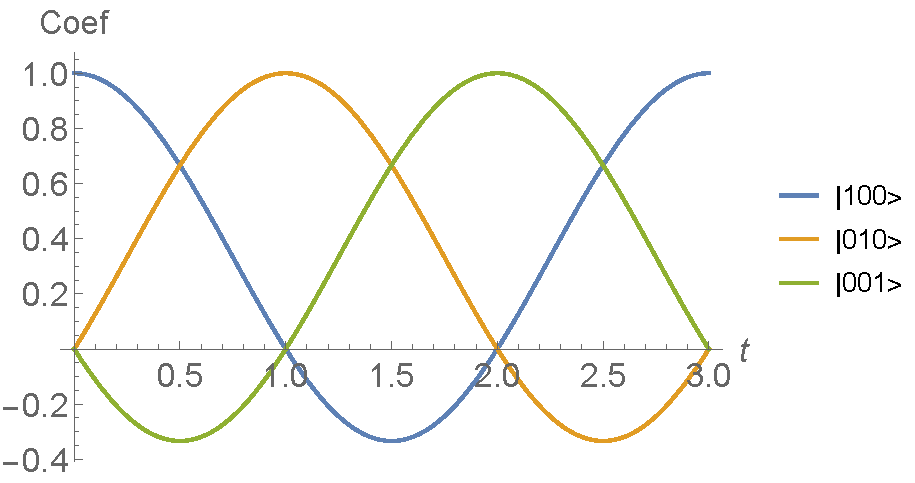
\includegraphics[width=.5\textwidth]{timeevol}
	\caption{Evolution of coefficients if the system starts in state $\ket{100}$.}
	\label{fig:timeevol}
\end{figure}

\section{Multi-Site Hamiltonian}

For a chain of $2n+1$ spins, we can define a similar hamiltonian by putting the 3-site hamiltonian on sites 1-3, sites 3-5, etc. For $n=1$, this is
\begin{align}
H_5 = H_3\otimes\mathbb{I}_2 + \mathbb{I}_2\otimes H_3.
\end{align} 
This hamiltonian still preserves total spin. 

Starting in $\ket{00001}$, the coefficients follow the pattern of figure~\ref{fig:timeevol5}. At first the evolution is similar to the $n=1$ case, with $\ket{10000}$ and then $\ket{01000}$ reaching near maximal. The coefficient of $\ket{00001}$ is 
\begin{align}
\frac{1}{10} \left(3 \cos \left(\frac{2}{3} \sqrt{\frac{5}{3}} \pi  t\right)+5 \cos \left(\frac{2 \pi  t}{3 \sqrt{3}}\right)+2\right)
\end{align} 
which is shown in figure~\ref{fig:onecoef}. Although it appears to be quasi-periodic, it cannot ever reach 1 for $t\ne 0$ or be truly periodic because its time coefficients are not rationally related.

\begin{figure}
	\centering
	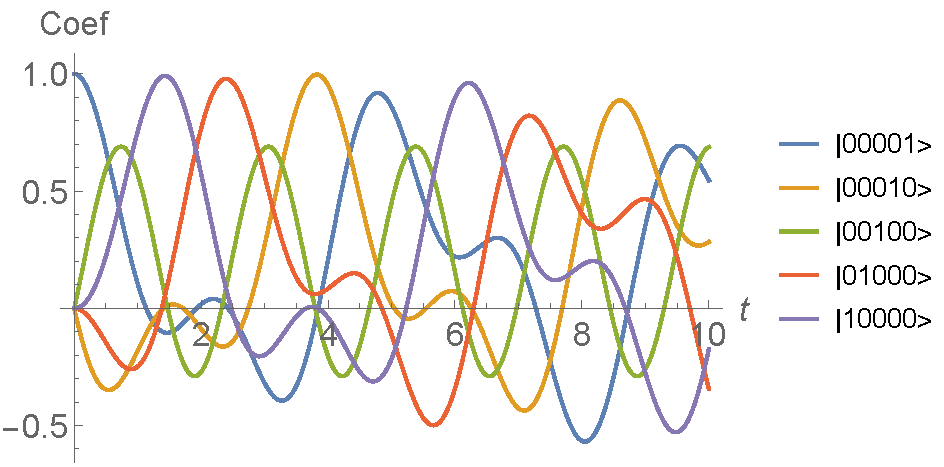
\includegraphics[width=.5\textwidth]{timeevol5}
	\caption{Evolution of coefficients if the system starts in state $\ket{00001}$.}
	\label{fig:timeevol5}
\end{figure}

\begin{figure}
	\centering
	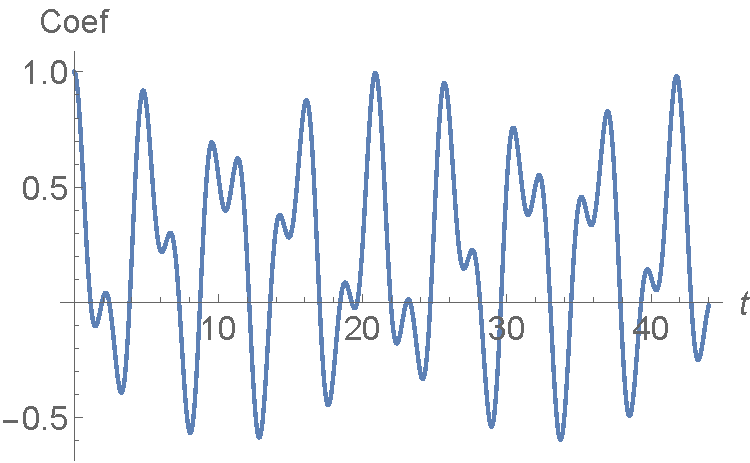
\includegraphics[width=.5\textwidth]{onecoef}
	\caption{Coefficient for $\ket{00001}$ when that is the starting state.}
	\label{fig:onecoef}
\end{figure}

The coefficient for $\ket{00100}$ does not fit the pattern. It does not reach maximum at the right time and it does have a periodic structure. Furthermore, when the starting state is $\ket{00010}$ the problematic state is still $\ket{00100}$, probably because of the chaining mechanism. When the starting state is $\ket{00100}$ the coefficients for $\ket{10000}$ and $\ket{00001}$ always vanish. The next chaining method to try will be to have $2n$ spins, and to have the first spin complete the last trio.

\end{document}
